\subsection{Sequence diagrams}
The following sequence diagrams show the message flow between the AR, the PEP and the PDP.
The IDs of the EAP- and RADIUS-messages correspond to the provided Wireshark-captures.

\begin{figure}[ht]
 \centering
 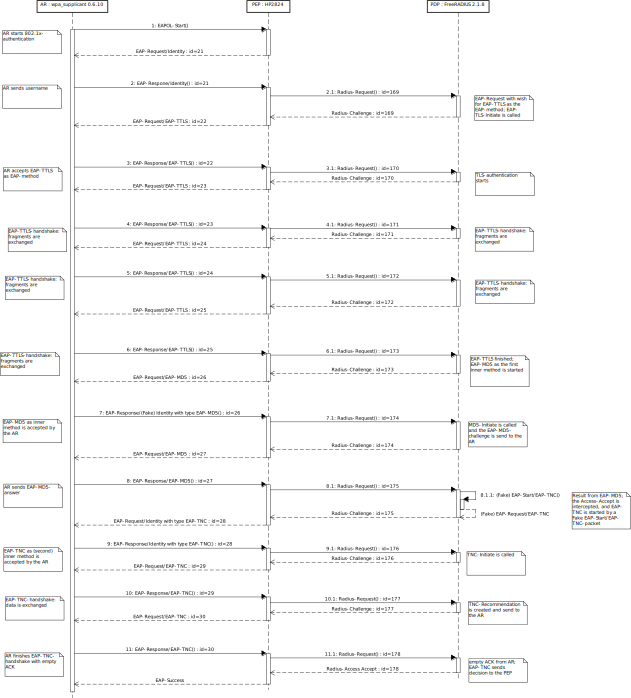
\includegraphics[width=\textwidth]{freeradius-eapttls-patch/diagrams/packet-flow-complete.png}
% 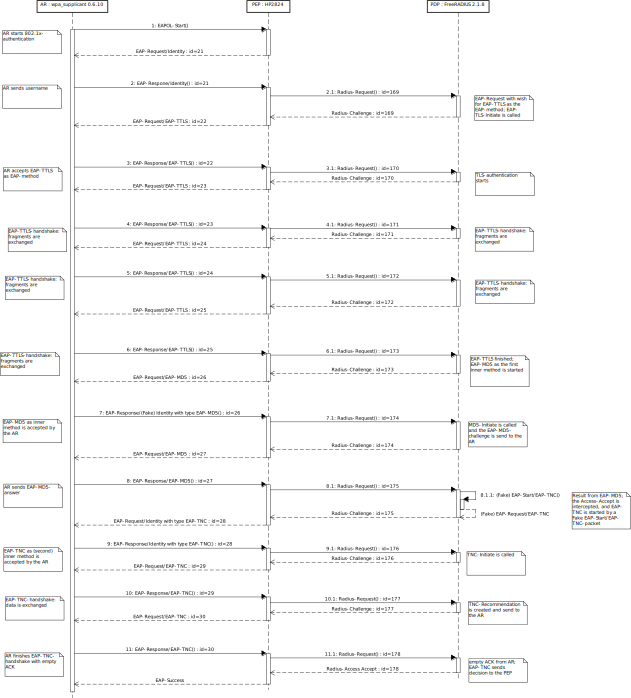
\includegraphics[width=\textwidth]{freeradius-eapttls-patch/diagrams/packet-flow-complete.pdf}
 \caption{EAP TTLS patch packet flow}
 \label{fig:eapttls-patch-flow-1}
\end{figure}

\subsubsection*{Remarks}
The (fake) EAP-Response/Identity of the AR in the EAP-packet with ID 26 is created by wpa\_supplicant.
As a response to the end of the TLS-authentication, a fake EAP-Request/Identity is created inside of wpa\_supplicant,
to start the inner method.
The following debug-output is from wpa\_supplicant, showing this behaviour.

\begin{lstlisting}[style=eapttls-config]
EAP: Received EAP-Request id=26 method=21 vendor=0 vendorMethod=0
...
EAP-TTLS: TLS done, proceed to Phase 2
EAP-TTLS: Derived key - hexdump(len=64): [REMOVED]
EAP-TTLS: received 0 bytes encrypted data for Phase 2
EAP-TTLS: empty data in beginning of Phase 2 - use fake EAP-Request Identity
EAP-TTLS: Phase 2 EAP Request: type=1
EAP: using real identity - hexdump_ascii(len=7):
     74 6e 63 75 73 65 72                              tncuser
EAP-TTLS: AVP encapsulate EAP Response - hexdump(len=12): 02 00 00 0c 01 74 6e 63 75 73 65 72
\end{lstlisting}

\clearpage